\section{Summary}\label{sec:summary}
This experiment uses a Lab-Volt 5250 robotic arm (see Figure ~\ref{fig:arm}) to demonstrate the differences between angular, linear and GUI control modes.
\begin{figure}[tbph]
  \centering
  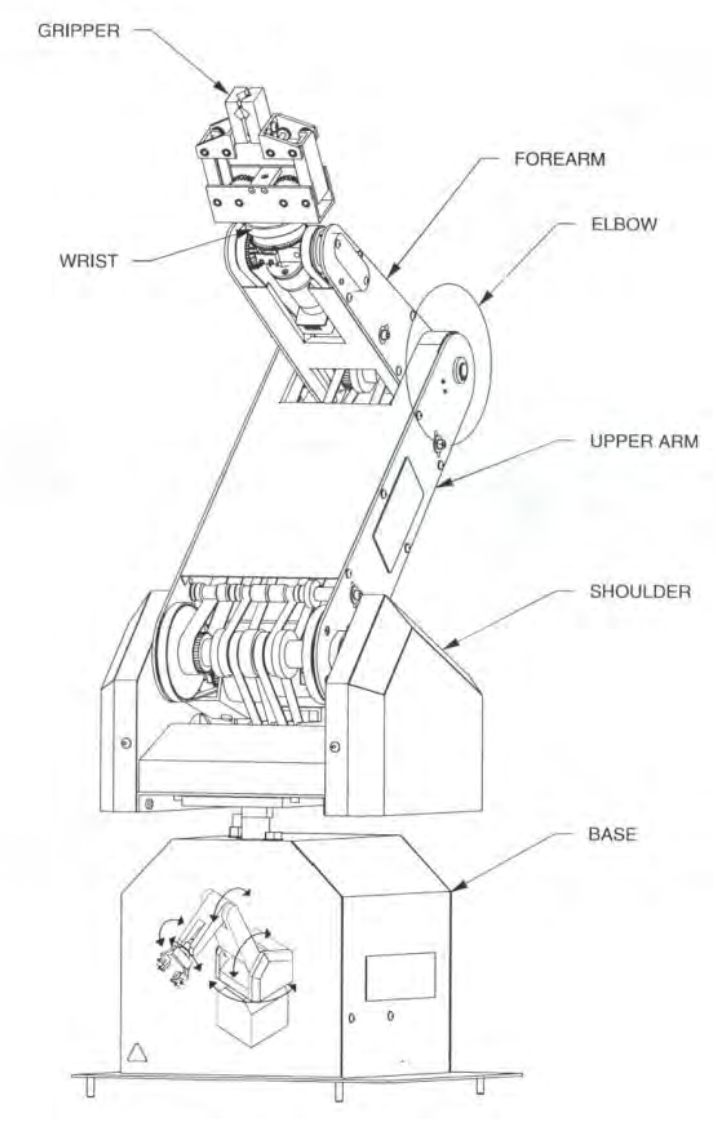
\includegraphics[width=0.4\linewidth]{graphics/arm}
  \caption{Lab-Volt 5250 robotic arm}
  \label{fig:arm}
\end{figure}

Angular and GUI modes allow the user to control the position of each robot joint.
Linear mode moves the tip of the robot's gripper through a Cartesian plane and determines the specific joint movements needed to achieve this motion.
